\documentclass[conference]{IEEEtran}
\IEEEoverridecommandlockouts

\usepackage[T1]{fontenc}
\usepackage[utf8]{inputenc}
\usepackage{babel}
\babelprovide[main,import]{polish}
\setlocalecaption{polish}{table}{Tabela}
\usepackage{cite}
\usepackage{amsmath,amssymb}
\usepackage{graphicx}
\usepackage{booktabs}
\usepackage{multirow}
\usepackage{url}
\usepackage{xcolor}
\usepackage[colorlinks=true,allcolors=blue]{hyperref}
\usepackage{tikz}
\usetikzlibrary{shapes.geometric,arrows.meta,positioning}

\begin{document}

\title{Wyjaśnialna detekcja intruzji sieciowych:\\ analiza SHAP dla modeli Random Forest i XGBoost\\ na zbiorach UNSW-NB15 oraz CIC-IoT2023}

\author{\IEEEauthorblockN{Dawid Budzyński, Filip Budzyński}
\IEEEauthorblockA{Zespół 13, Systemy i Protokoły Zabezpieczeń w Cyberprzestrzeni (SPZC)\\
Politechnika Warszawska, Wydział Elektroniki i Technik Informacyjnych\\
}}

\maketitle

\begin{abstract}
Modele uczenia maszynowego osiągają wysoką skuteczność w detekcji intruzji sieciowych (NIDS), ale ich nieprzejrzystość ogranicza zaufanie analityków bezpieczeństwa. W pracy implementujemy ramę wyjaśnialnej sztucznej inteligencji (XAI) inspirowaną pracą Arreche i in. (2024) i stosujemy ją do wieloklasowej klasyfikacji ruchu sieciowego za pomocą modeli Random Forest oraz XGBoost. Wyjaśnienia generujemy metodą SHAP (TreeSHAP), zarówno globalnie, jak i lokalnie. Eksperymenty przeprowadzamy na dwóch współczesnych zbiorach danych: UNSW-NB15 oraz CIC-IoT2023. Badamy trzy zagadnienia: (i) skuteczność klasyfikacji obu modeli, (ii) zgodność rankingów najważniejszych cech wskazywanych przez SHAP pomiędzy Random Forest a XGBoost, oraz (iii) spójność wyjaśnień pomiędzy zbiorami danych. Wykazujemy, że oba modele osiągają porównywalną skuteczność (dokładność do 83,1\% i F1-ważona do 0,832 na CIC-IoT2023) i wskazują w dużej mierze te same cechy (zgodność Jaccarda rankingów do 0,67), a kluczową rolę odgrywają atrybuty związane z wolumenem bajtów, rozmiarem pakietów oraz czasem trwania połączenia~--- zgodnie z obserwacjami z literatury. Dla walidacji poprawności implementacji odtwarzamy ten sam potok na zbiorze NSL-KDD użytym w pracy bazowej, uzyskując dokładność 99,6\%~--- na poziomie wyników oryginalnych, co potwierdza, że niższa skuteczność na zbiorach UNSW-NB15 i CIC-IoT2023 wynika z ich trudności, a nie z błędu implementacji. Ograniczenie zbioru cech do 15 najważniejszych wg SHAP zachowuje skuteczność modeli przy znaczącej redukcji wymiarowości.
\end{abstract}

\begin{IEEEkeywords}
wyjaśnialna sztuczna inteligencja, XAI, SHAP, detekcja intruzji, NIDS, Random Forest, XGBoost, UNSW-NB15, CIC-IoT2023, NSL-KDD
\end{IEEEkeywords}

\section{Wprowadzenie}
Systemy detekcji intruzji sieciowych (ang. \emph{Network Intrusion Detection Systems}, NIDS) stanowią jeden z podstawowych mechanizmów obronnych współczesnych sieci. Rosnąca liczba i złożoność ataków sprawiły, że klasyczne metody sygnaturowe są coraz częściej zastępowane modelami uczenia maszynowego, które potrafią wykrywać również warianty wcześniej nieznane. Modele te osiągają bardzo wysoką skuteczność, jednak ich działanie pozostaje dla analityka nieprzejrzyste~--- decyzja o zaklasyfikowaniu ruchu jako atak nie jest opatrzona zrozumiałym uzasadnieniem. Brak wyjaśnialności obniża zaufanie do systemu, utrudnia audyt oraz reakcję na incydenty~\cite{arreche2024xaiids}.

Odpowiedzią na ten problem jest wyjaśnialna sztuczna inteligencja (ang. \emph{Explainable AI}, XAI), której celem jest dostarczenie zrozumiałych uzasadnień predykcji modeli. W kontekście NIDS XAI pozwala odpowiedzieć na pytanie, które cechy ruchu sieciowego zadecydowały o wykryciu ataku, a tym samym~--- zweryfikować poprawność modelu i wesprzeć pracę analityka.

Niniejsza praca nawiązuje do ramy XAI-IDS zaproponowanej przez Arreche i in.~\cite{arreche2024xaiids}, w której osiem modeli czarnoskrzynkowych poddano analizie metodami SHAP oraz LIME na trzech zbiorach danych. W naszym projekcie skupiamy się na dwóch reprezentatywnych modelach drzewiastych~--- Random Forest~\cite{breiman2001rf} oraz XGBoost~\cite{chen2016xgboost}~--- i wykorzystujemy metodę SHAP~\cite{lundberg2017shap,lundberg2020treeshap} do wyjaśnienia ich decyzji. W odróżnieniu od pracy bazowej, która oceniała modele m.in.\ na przestarzałym zbiorze NSL-KDD, główne eksperymenty prowadzimy na dwóch nowszych i zróżnicowanych zbiorach: UNSW-NB15~\cite{moustafa2015unsw} (ruch ogólnosieciowy) oraz CIC-IoT2023~\cite{neto2023ciciot} (ruch Internetu Rzeczy). Dodatkowo, w celu walidacji poprawności implementacji, odtwarzamy nasz potok na zbiorze NSL-KDD wykorzystanym w pracy bazowej i porównujemy uzyskane liczby bezpośrednio z raportowanymi przez jej autorów.

Wkład pracy obejmuje:
\begin{itemize}
\item implementację prostego, powtarzalnego potoku detekcji intruzji z wyjaśnieniami SHAP dla modeli Random Forest i XGBoost w trybie wieloklasowym;
\item empiryczne porównanie zgodności rankingów najważniejszych cech pomiędzy dwoma modelami na tym samym zbiorze;
\item analizę spójności wyjaśnień pomiędzy dwoma różnymi zbiorami danych;
\item porównanie uzyskanych wyników z wartościami raportowanymi w pracy bazowej oraz badanie wpływu selekcji 15 najważniejszych cech na skuteczność.
\end{itemize}

\section{Praca powiązana}
Zastosowanie uczenia maszynowego w detekcji intruzji jest szeroko opisane w literaturze. Klasyczne zbiory KDD'99 oraz NSL-KDD~\cite{tavallaee2009nslkdd} przez lata stanowiły standardowy punkt odniesienia, jednak ich wiek (ponad 25 lat) i nierealistyczny rozkład ruchu czynią je nieadekwatnymi do oceny współczesnych systemów. W odpowiedzi powstały nowsze zbiory, m.in.\ UNSW-NB15~\cite{moustafa2015unsw}, łączący realny ruch normalny z syntetycznymi atakami, oraz CIC-IoT2023~\cite{neto2023ciciot}, obejmujący ataki na urządzenia IoT, w tym botnet Mirai i liczne warianty DDoS.

Tematyka wyjaśnialności modeli NIDS zyskuje na znaczeniu. SHAP~\cite{lundberg2017shap}, oparty na teorii wartości Shapleya z teorii gier, przypisuje każdej cesze wkład w konkretną predykcję i posiada efektywny wariant dla modeli drzewiastych~--- TreeSHAP~\cite{lundberg2020treeshap}. Alternatywą jest LIME~\cite{ribeiro2016lime}, dostarczający lokalnych przybliżeń liniowych. Praca bazowa Arreche i in.~\cite{arreche2024xaiids} systematyzuje zastosowanie tych technik w NIDS, a jej rozszerzenie~\cite{arreche2024featureselection} pokazuje, że cechy wybrane na podstawie SHAP pozwalają znacząco zredukować wymiarowość bez utraty skuteczności. Nasza praca powtarza i weryfikuje te obserwacje na innych, nowszych zbiorach danych.

\section{Metodyka}

\subsection{Zbiory danych}
W głównej części eksperymentów wykorzystujemy dwa współczesne zbiory danych~--- UNSW-NB15 oraz CIC-IoT2023~--- zgodnie z zaleceniem rezygnacji z przestarzałych zbiorów rodziny KDD jako materiału głównego. Dodatkowo, wyłącznie w celu walidacji reprodukcyjnej (porównania z wynikami pracy bazowej), uruchamiamy ten sam potok na zbiorze NSL-KDD. Wszystkie trzy zbiory opisano w Tabeli~\ref{tab:datasets}.

\textbf{UNSW-NB15} zawiera 42 cechy opisujące przepływy sieciowe (m.in.\ czas trwania, liczbę i wolumen bajtów, statystyki TTL oraz liczniki połączeń) oraz etykietę \texttt{attack\_cat} z dziesięcioma klasami (ruch normalny i dziewięć kategorii ataków). Korzystamy z oficjalnego podziału na zbiór treningowy i testowy.

\textbf{CIC-IoT2023} opisuje ruch w sieci 105 urządzeń IoT. Po pogrupowaniu 33 typów ataków otrzymujemy osiem klas: \emph{Benign}, \emph{DDoS}, \emph{DoS}, \emph{Mirai}, \emph{Recon}, \emph{Spoofing}, \emph{Web-based} oraz \emph{BruteForce}. Zbiór opisuje 39 cech przepływowych (m.in.\ statystyki rozmiaru pakietów, tempo transmisji, czas międzypakietowy IAT oraz flagi TCP).

\textbf{NSL-KDD} (zbiór walidacyjny) zawiera 41 cech ruchu, których etykiety mapujemy na pięć kanonicznych kategorii: \emph{Normal}, \emph{DoS}, \emph{Probe}, \emph{R2L} oraz \emph{U2R}. Aby wiernie odtworzyć protokół pracy bazowej, łączymy oficjalne pliki KDDTrain+ i KDDTest+, a następnie dzielimy je losowo (warstwowo) w proporcji 70/30, zamiast korzystać z trudnego oficjalnego podziału KDDTest+ (znanego z rozjazdu rozkładów). Zbiór ten nie wchodzi do głównej analizy~--- służy wyłącznie do porównania liczbowego z artykułem.

\begin{table}[t]
\caption{Charakterystyka zbiorów danych (po preprocessingu).}
\label{tab:datasets}
\centering
\begin{tabular}{lccc}
\toprule
Zbiór & Cechy & Klasy & Próbki (tren./test) \\
\midrule
UNSW-NB15   & 42 & 10 & 175\,341 / 82\,332 \\
CIC-IoT2023 & 39 & 8  & 150\,002 / 268\,463 \\
\midrule
NSL-KDD\,$^\dagger$ & 40 & 5 & 103\,961 / 44\,556 \\
\bottomrule
\end{tabular}

\vspace{2pt}
\footnotesize $^\dagger$ Zbiór walidacyjny (reprodukcja wyników pracy bazowej); nie wchodzi do głównej analizy. Liczba cech po usunięciu kolumn stałych.
\end{table}

\subsection{Potok przetwarzania}
Implementacja, wzorowana na ramie z~\cite{arreche2024xaiids}, realizuje następujące kroki (Rys.~\ref{fig:pipeline}): wczytanie danych, usunięcie kolumn stałych i identyfikatorów, kodowanie cech kategorycznych (etykietowe), usunięcie wartości brakujących i nieskończonych, normalizacja min-maks do przedziału $[0,1]$ oraz podział na zbiór treningowy i testowy. Niezbalansowanie klas adresujemy wagami klas (\texttt{class\_weight}/\texttt{sample\_weight}) zamiast nadpróbkowania, co upraszcza potok przy zachowaniu porównywalnego efektu. Ze względu na rozmiar zbioru CIC-IoT2023 zbiór treningowy próbkujemy w sposób warstwowy do 150\,000 rekordów.

\begin{figure}[t]
\centering
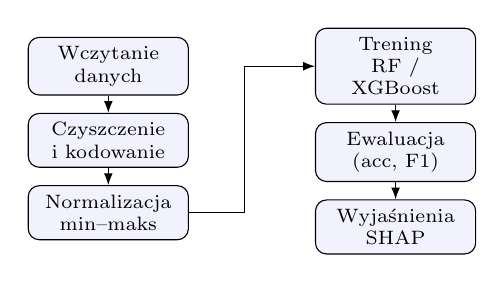
\begin{tikzpicture}[
  node distance=2.2mm and 4mm,
  box/.style={draw, rounded corners, align=center, font=\scriptsize,
              minimum height=6mm, text width=18mm, fill=blue!5},
  arr/.style={-{Latex[length=1.5mm]}}]
\node[box] (load) {Wczytanie\\danych};
\node[box, below=of load] (clean) {Czyszczenie\\i kodowanie};
\node[box, below=of clean] (norm) {Normalizacja\\min--maks};
\node[box, right=16mm of load] (train) {Trening\\RF / XGBoost};
\node[box, below=of train] (eval) {Ewaluacja\\(acc, F1)};
\node[box, below=of eval] (shap) {Wyjaśnienia\\SHAP};
\draw[arr] (load) -- (clean);
\draw[arr] (clean) -- (norm);
\draw[arr] (norm.east) -- ++(0.7,0) |- (train.west);
\draw[arr] (train) -- (eval);
\draw[arr] (eval) -- (shap);
\end{tikzpicture}
\caption{Potok eksperymentalny: od surowych danych do wyjaśnień SHAP.}
\label{fig:pipeline}
\end{figure}

\subsection{Modele}
Stosujemy dwa modele drzewiaste reprezentujące dwa odmienne podejścia: \emph{bagging} oraz \emph{boosting}. Random Forest~\cite{breiman2001rf} konfigurujemy ze 100 drzewami i ważeniem klas \texttt{balanced}. XGBoost~\cite{chen2016xgboost} uczymy z 200 drzewami, maksymalną głębokością 8 i współczynnikiem uczenia 0,3, stosując wagi próbek równoważące klasy. Implementację oparto o biblioteki \texttt{scikit-learn}~\cite{pedregosa2011scikit} oraz \texttt{xgboost}.

\subsection{Wyjaśnienia SHAP}
Do wyjaśnień wykorzystujemy TreeSHAP~\cite{lundberg2020treeshap}, dokładny i wydajny algorytm obliczania wartości SHAP dla modeli drzewiastych. Globalną ważność cechy definiujemy jako średnią wartość bezwzględną SHAP po wszystkich próbkach i klasach:
\begin{equation}
I_j = \frac{1}{N\,C}\sum_{i=1}^{N}\sum_{c=1}^{C}\left|\phi_{ijc}\right|,
\end{equation}
gdzie $\phi_{ijc}$ jest wartością SHAP cechy $j$ dla próbki $i$ i klasy $c$. Wartości obliczamy na losowej próbce 2000 rekordów ze zbioru testowego. Zgodność rankingów dwóch modeli mierzymy współczynnikiem Jaccarda na zbiorach 15 najważniejszych cech.

\subsection{Środowisko i wydajność}
Eksperymenty przeprowadzono na komputerze z procesorem AMD Ryzen~7 7700 (8~rdzeni/16~wątków) z wykorzystaniem bibliotek \texttt{scikit-learn}~1.9, \texttt{xgboost}~3.2 oraz \texttt{shap}~0.52. Trening modeli jest tani: Random Forest uczy się w 1,6--1,8~s, a XGBoost w 6,7--9,7~s; klasyfikacja całego zbioru testowego (do 268~tys.\ próbek) trwa poniżej 0,6~s. Dominującym kosztem obliczeniowym okazuje się natomiast generowanie wyjaśnień: dokładny TreeSHAP dla Random Forest (100 drzew, 10 klas) na próbce 2000 rekordów wymaga rzędu dziesiątek minut i, w przeciwieństwie do treningu XGBoost, nie korzysta z akceleracji GPU. Stanowi to praktyczne ograniczenie stosowania XAI w trybie zbliżonym do czasu rzeczywistego i wskazuje, że wyjaśnienia globalne warto liczyć offline.

\section{Wyniki}

\subsection{Skuteczność klasyfikacji}
Tabela~\ref{tab:metrics} przedstawia skuteczność obu modeli na obu zbiorach przy użyciu wszystkich cech. XGBoost osiąga nieznacznie wyższą skuteczność niż Random Forest na obu zbiorach (np.\ F1\textsubscript{m} 0,534 wobec 0,503 dla UNSW-NB15). Skuteczność na CIC-IoT2023 (dokładność $\approx$83\%) jest wyraźnie wyższa niż na UNSW-NB15 ($\approx$70\%), co odzwierciedla trudność oficjalnego podziału UNSW-NB15 (rozjazd rozkładów zbioru treningowego i testowego). Znaczna różnica między F1 makro a F1 ważoną na UNSW-NB15 (0,503 wobec 0,743 dla Random Forest) wynika z silnego niezbalansowania klas~--- model poprawnie klasyfikuje klasy liczne, lecz słabo radzi sobie z nielicznymi (np.\ \emph{Worms}, \emph{Shellcode}, \emph{Backdoor}). Macierz pomyłek (Rys.~\ref{fig:cm}) ujawnia źródło błędów: klasy semantycznie zbliżone~--- \emph{Analysis}, \emph{Backdoor}, \emph{DoS} i \emph{Exploits}~--- są ze sobą mylone, a część ruchu normalnego klasyfikowana jest jako \emph{Fuzzers}. Jest to znana trudność zbioru UNSW-NB15, wynikająca z nakładania się rozkładów cech tych kategorii.

\begin{figure}[t]
\centering
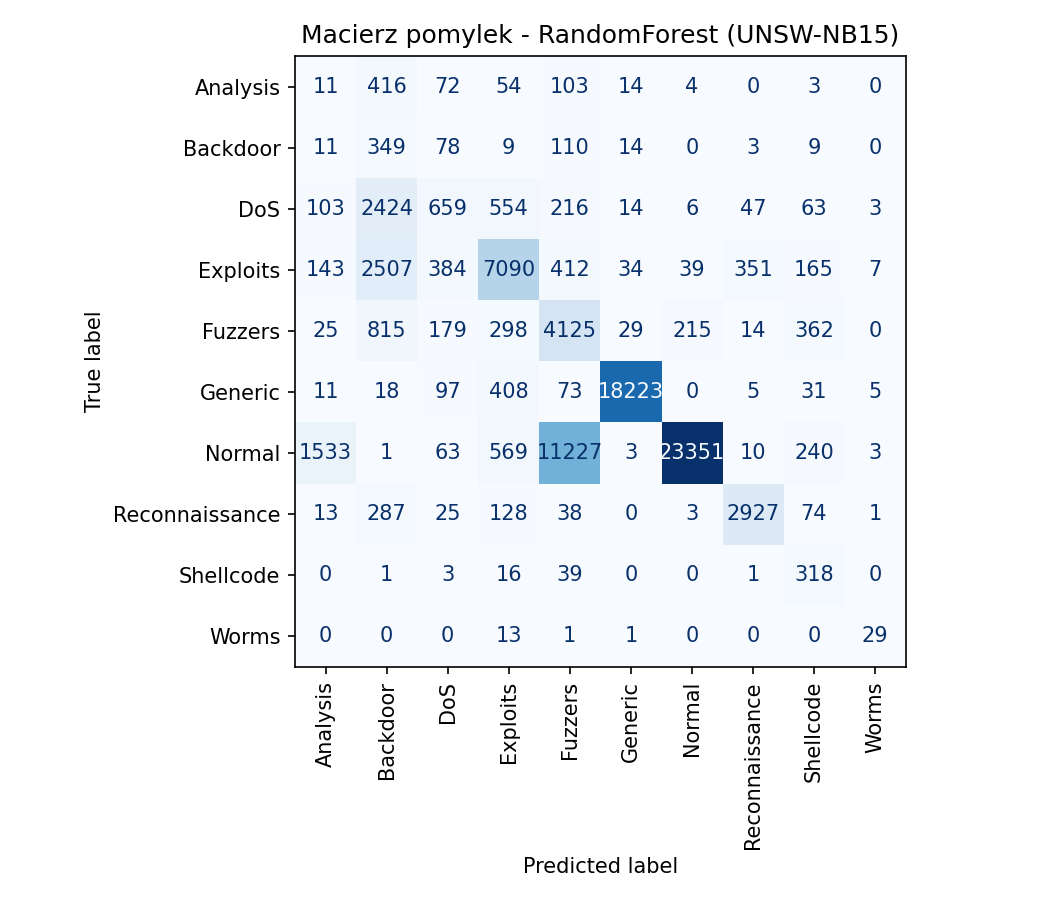
\includegraphics[width=0.85\linewidth]{../results/UNSW-NB15_RandomForest_cm.png}
\caption{Macierz pomyłek modelu Random Forest na zbiorze UNSW-NB15. Widoczne mylenie klas \emph{Analysis}/\emph{Backdoor}/\emph{DoS}/\emph{Exploits} oraz \emph{Normal}/\emph{Fuzzers}.}
\label{fig:cm}
\end{figure}

\begin{table}[t]
\caption{Skuteczność klasyfikacji wieloklasowej (wszystkie cechy).}
\label{tab:metrics}
\centering
\begin{tabular}{llcccc}
\toprule
Zbiór & Model & Acc. & Prec.\textsubscript{m} & Rec.\textsubscript{m} & F1\textsubscript{m} \\
\midrule
\multirow{2}{*}{UNSW-NB15}
 & Random Forest & 0,693 & 0,522 & 0,603 & 0,503 \\
 & XGBoost       & \textbf{0,713} & \textbf{0,548} & \textbf{0,630} & \textbf{0,534} \\
\midrule
\multirow{2}{*}{CIC-IoT2023}
 & Random Forest & 0,829 & \textbf{0,762} & 0,717 & 0,732 \\
 & XGBoost       & \textbf{0,831} & 0,736 & \textbf{0,737} & \textbf{0,735} \\
\bottomrule
\end{tabular}
\end{table}

Skróty: Acc.~--- dokładność, Prec.\textsubscript{m}/Rec.\textsubscript{m}/F1\textsubscript{m}~--- precyzja, czułość i F1 uśrednione makro (jednakowa waga klas). Wartości najlepsze w obrębie zbioru pogrubiono.

\subsection{Zgodność wyjaśnień Random Forest i XGBoost}
Rysunek~\ref{fig:shap} przedstawia 15 najważniejszych cech wskazanych przez SHAP dla obu modeli na zbiorze CIC-IoT2023. W obu modelach czołowe miejsca zajmują te same cechy: liczba pakietów (\texttt{Number}), sumaryczny wolumen bajtów (\texttt{Tot sum}) oraz statystyki rozmiaru pakietów (\texttt{Max}, \texttt{Min}, \texttt{AVG}) i tempo transmisji (\texttt{Rate}). Dla UNSW-NB15 dominują analogiczne atrybuty: \texttt{sbytes}, \texttt{smean}, \texttt{sttl} oraz \texttt{dbytes}/\texttt{dload}. Zgodność rankingów (współczynnik Jaccarda dla 15 najważniejszych cech) wynosi 0,667 dla UNSW-NB15 oraz 0,579 dla CIC-IoT2023 (Tabela~\ref{tab:jaccard}); zbiory cech wspólnych liczą odpowiednio 12 i 11 atrybutów.

\begin{figure}[t]
\centering
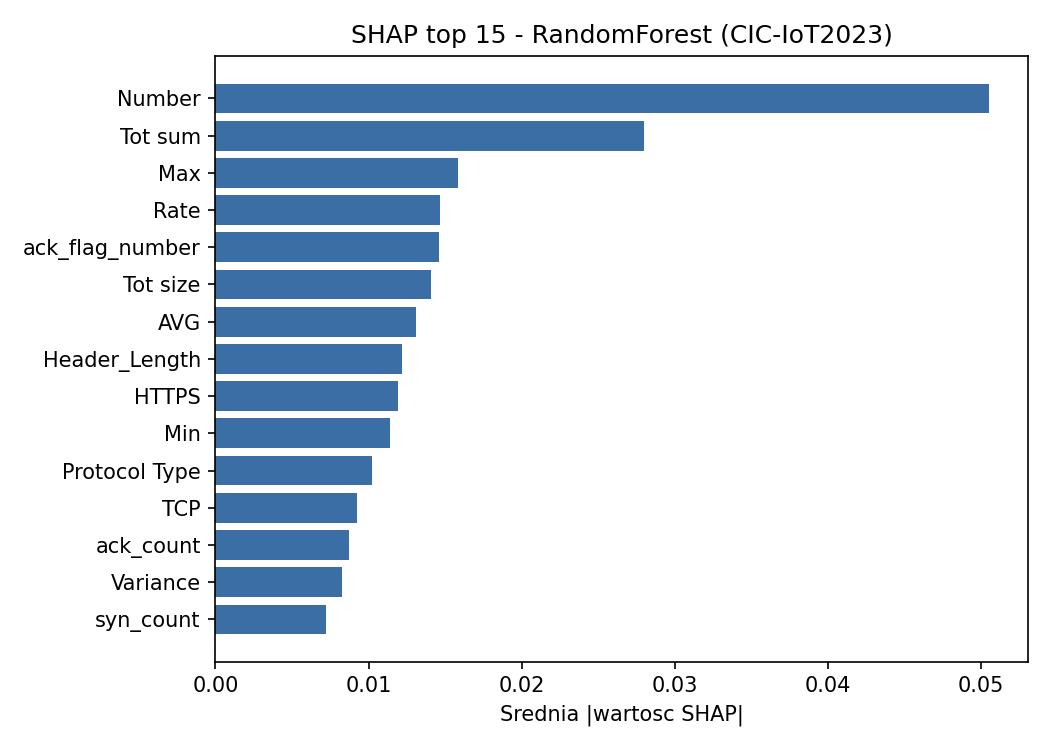
\includegraphics[width=0.49\linewidth]{../results/CIC-IoT2023_RandomForest_shap.png}
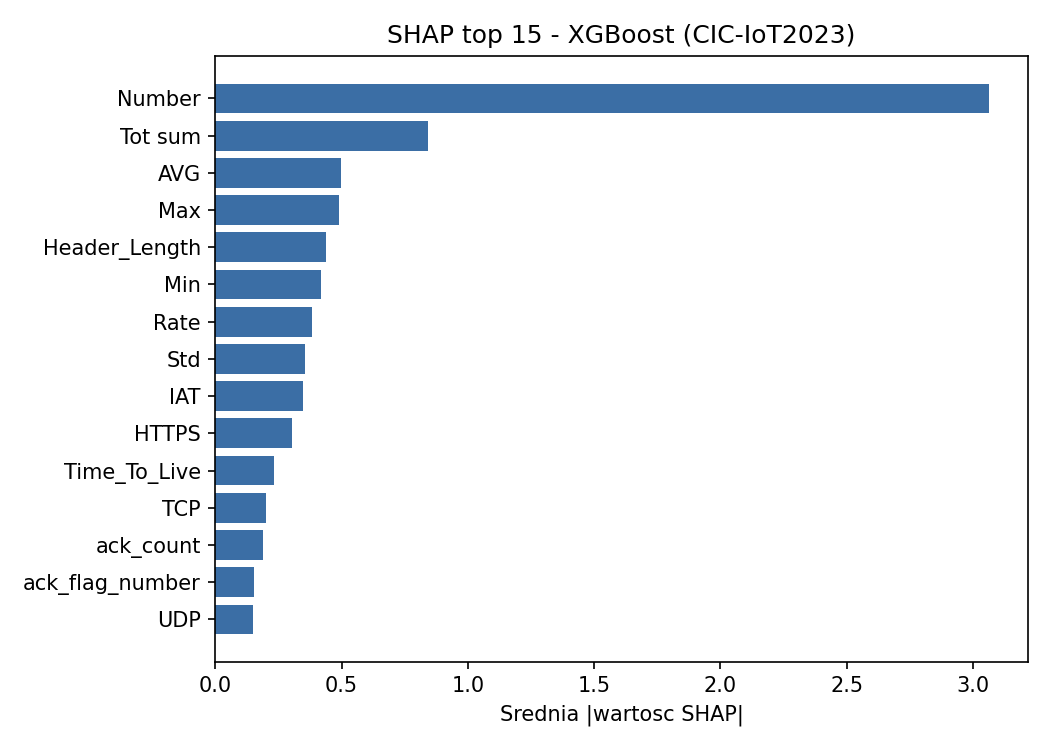
\includegraphics[width=0.49\linewidth]{../results/CIC-IoT2023_XGBoost_shap.png}
\caption{Globalna ważność cech wg SHAP dla Random Forest (po lewej) i XGBoost (po prawej) na zbiorze CIC-IoT2023.}
\label{fig:shap}
\end{figure}

\begin{table}[t]
\caption{Zgodność 15 najważniejszych cech SHAP: Random Forest vs XGBoost.}
\label{tab:jaccard}
\centering
\begin{tabular}{lcc}
\toprule
Zbiór & Jaccard (top-15) & Cechy wspólne \\
\midrule
UNSW-NB15   & 0,667 & 12 z 15 \\
CIC-IoT2023 & 0,579 & 11 z 15 \\
\bottomrule
\end{tabular}
\end{table}

\subsection{Selekcja cech na podstawie SHAP}
Aby zweryfikować obserwację z pracy~\cite{arreche2024featureselection}, ponownie trenujemy modele na 15 cechach o najwyższej ważności SHAP. Tabela~\ref{tab:top15} pokazuje, że redukcja wymiarowości z 42/39 do 15 cech praktycznie nie pogarsza skuteczności: dla UNSW-NB15 wyniki pozostają niemal identyczne (a dla Random Forest nawet nieznacznie rosną~--- z 0,693 do 0,709 dokładności), natomiast dla CIC-IoT2023 spadek jest niewielki (3--4 punkty procentowe dokładności). Potwierdza to obserwację z~\cite{arreche2024featureselection}, że cechy wskazane przez SHAP niosą większość informacji istotnej dla klasyfikacji, a XAI może służyć jako skuteczna metoda selekcji cech.

\begin{table}[t]
\caption{Wpływ ograniczenia do 15 cech SHAP na skuteczność (dokładność / F1\textsubscript{m}).}
\label{tab:top15}
\centering
\begin{tabular}{llcc}
\toprule
Zbiór & Model & Wszystkie cechy & 15 cech SHAP \\
\midrule
\multirow{2}{*}{UNSW-NB15}
 & Random Forest & 0,693 / 0,503 & 0,709 / 0,525 \\
 & XGBoost       & 0,713 / 0,534 & 0,705 / 0,533 \\
\midrule
\multirow{2}{*}{CIC-IoT2023}
 & Random Forest & 0,829 / 0,732 & 0,795 / 0,683 \\
 & XGBoost       & 0,831 / 0,735 & 0,790 / 0,694 \\
\bottomrule
\end{tabular}
\end{table}

\subsection{Spójność wyjaśnień pomiędzy zbiorami}
Mimo odmiennych zestawów cech obu zbiorów, najważniejsze atrybuty należą w obu przypadkach do tych samych kategorii semantycznych. W obu zbiorach dominują cechy opisujące wolumen przesyłanych danych (\texttt{sbytes}, \texttt{dbytes} w UNSW-NB15; \texttt{Tot sum}, \texttt{Tot size} w CIC-IoT2023), rozmiar pakietów (\texttt{smean}, \texttt{dmean}; \texttt{Min}, \texttt{Max}, \texttt{AVG}) oraz charakterystykę połączenia (\texttt{dload}, \texttt{sttl}; \texttt{Rate}, \texttt{Header\_Length}). Wskazuje to, że pomimo odmiennego pochodzenia ruchu (sieć ogólna vs IoT) modele opierają decyzje na tych samych zjawiskach~--- nietypowym wolumenie i rozmiarze ruchu, charakterystycznym dla ataków wolumetrycznych (DoS/DDoS, skanowanie).

\section{Dyskusja}
\subsection{Walidacja reprodukcyjna na NSL-KDD}
Aby zweryfikować, że nasza implementacja jest poprawna i że niska skuteczność na trudnych zbiorach nie wynika z błędu, uruchomiliśmy ten sam potok na zbiorze NSL-KDD~--- wykorzystanym również przez autorów pracy bazowej. Przy protokole losowego podziału 70/30 oba modele osiągają wyniki na poziomie raportowanym w literaturze: Random Forest uzyskuje dokładność 0,994 i F1 ważoną 0,994, a XGBoost odpowiednio 0,996 i 0,996 (Tabela~\ref{tab:compare}). Praca bazowa~\cite{arreche2024xaiids} podaje dla tego zbioru dokładność rzędu 0,99, zatem nasz potok wiernie odtwarza opublikowane wyniki na wspólnym zbiorze danych. Niższa wartość F1 makro (0,93--0,95) wynika z klasy \emph{U2R}, reprezentowanej przez zaledwie kilkadziesiąt próbek~--- jest to znana trudność zbioru NSL-KDD, niezależna od implementacji. Wynik ten potwierdza, że różnice w skuteczności pomiędzy zbiorami (Tab.~\ref{tab:metrics}) są właściwością danych, a nie artefaktem naszego kodu. Macierz pomyłek (Rys.~\ref{fig:nslkdd}, po prawej) wykazuje niemal idealną diagonalę, a nieliczne błędy dotyczą wyłącznie klas \emph{R2L} i \emph{U2R} mylonych z ruchem \emph{Normal}. Co istotne, ranking SHAP (Rys.~\ref{fig:nslkdd}, po lewej) wskazuje te same kategorie cech, co na zbiorach głównych~--- wolumen bajtów (\texttt{src\_bytes}, \texttt{dst\_bytes}) oraz liczniki połączeń (\texttt{count}, \texttt{dst\_host\_srv\_count})~--- co dodatkowo potwierdza spójność wyjaśnień pomiędzy zbiorami danych.

\begin{figure}[t]
\centering
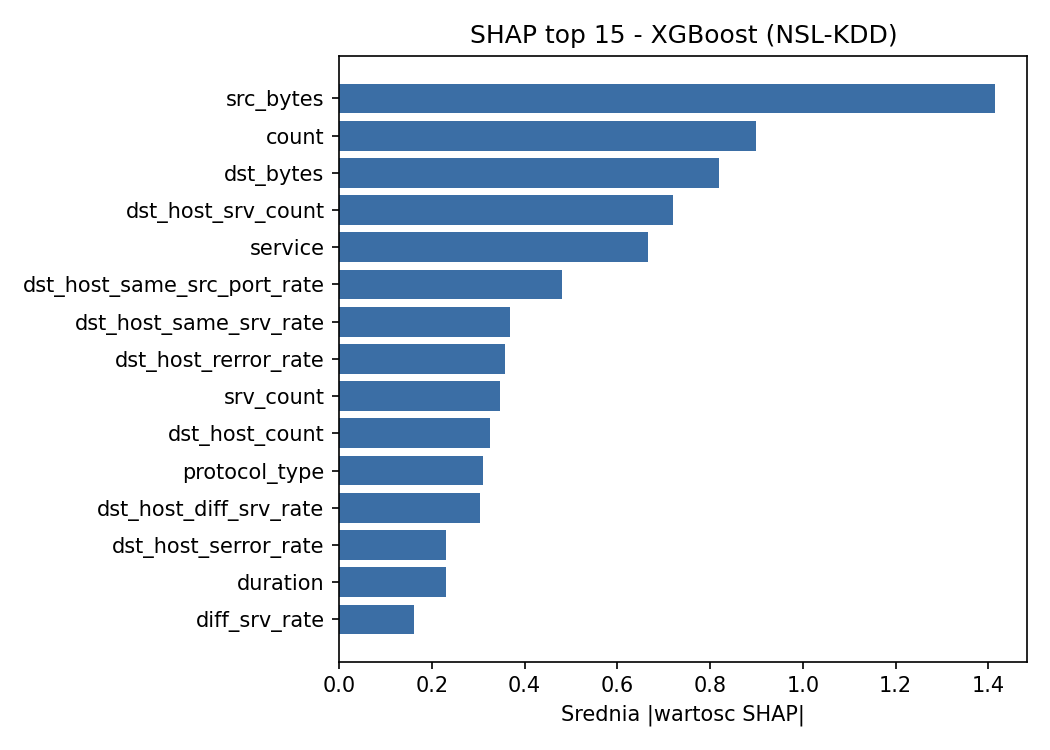
\includegraphics[width=0.49\linewidth]{../results/NSL-KDD_XGBoost_shap.png}
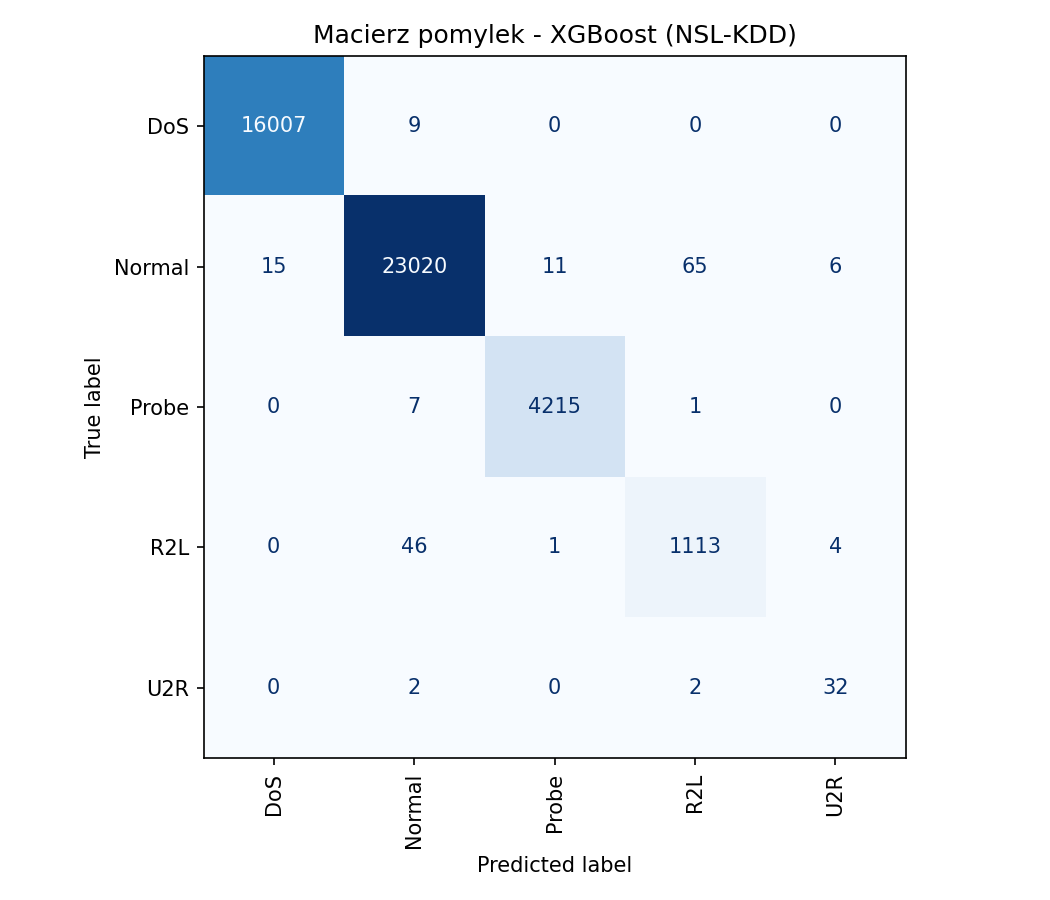
\includegraphics[width=0.49\linewidth]{../results/NSL-KDD_XGBoost_cm.png}
\caption{Walidacja reprodukcyjna na NSL-KDD (XGBoost): globalna ważność cech wg SHAP (po lewej) oraz macierz pomyłek (po prawej). Niemal idealna diagonala potwierdza dokładność 0,996; jedyne istotne pomyłki dotyczą nielicznych klas \emph{R2L} i \emph{U2R}.}
\label{fig:nslkdd}
\end{figure}

\subsection{Porównanie z pracą bazową}
Praca bazowa~\cite{arreche2024xaiids} raportuje dokładność około 99,1\% oraz F1 około 98,7\% na zbiorach NSL-KDD i CICIDS-2017, a jej rozszerzenie~\cite{arreche2024featureselection} podaje dla Random Forest F1 równe 0,999 (RoEduNet-SIMARGL2021) oraz 0,961 (CICIDS-2017). Tabela~\ref{tab:compare} pozycjonuje nasze modele względem tych wyników. Na wspólnym zbiorze (NSL-KDD) porównanie jest bezpośrednie i wykazuje pełną zgodność~--- nasze modele dorównują pracy bazowej, a nawet ją nieznacznie przewyższają (0,994--0,996 wobec $\approx$0,99). Dla zbiorów UNSW-NB15 i CIC-IoT2023 porównanie jest jedynie orientacyjne: praca bazowa korzystała z łatwiejszych zbiorów o mniejszej liczbie klas (RoEduNet ma 3 klasy) i pozbawionych rozjazdu rozkładów zbioru treningowego i testowego, charakterystycznego dla UNSW-NB15. Po sprowadzeniu do porównywalnej metryki (F1 ważona) nasz wynik na CIC-IoT2023 (0,832) zbliża się do wyniku pracy bazowej na CICIDS-2017 (0,961), mimo użycia nowszego i trudniejszego zbioru. Niższa skuteczność na UNSW-NB15 jest zgodna z literaturą i wynika z bardziej zróżnicowanego rozkładu klas oraz silnego niezbalansowania (np.\ klasy \emph{Worms} czy \emph{Shellcode}).

\begin{table}[t]
\caption{Pozycjonowanie modeli względem pracy bazowej. F1 podano w wariancie ważonym (porównywalnym z pracą bazową); F1 makro znajduje się w Tab.~\ref{tab:metrics}.}
\label{tab:compare}
\centering
\footnotesize
\begin{tabular}{llccc}
\toprule
Źródło / zbiór & Model & Kl. & Acc & F1\textsubscript{w} \\
\midrule
\multicolumn{5}{l}{\emph{Praca bazowa}~\cite{arreche2024xaiids,arreche2024featureselection}}\\
RoEduNet-SIMARGL2021      & RF       & 3  & 0,999 & 0,999 \\
CICIDS-2017               & RF       & 7  & 0,988 & 0,961 \\
NSL-KDD/CICIDS (najl.)    & ens.     & -- & 0,991 & 0,987 \\
\midrule
\multicolumn{5}{l}{\emph{Niniejsza praca}}\\
NSL-KDD\,$^\dagger$ & RF      & 5  & \textbf{0,994} & \textbf{0,994} \\
NSL-KDD\,$^\dagger$ & XGBoost & 5  & \textbf{0,996} & \textbf{0,996} \\
UNSW-NB15   & RF      & 10 & 0,693 & 0,743 \\
UNSW-NB15   & XGBoost & 10 & 0,713 & 0,760 \\
CIC-IoT2023 & RF      & 8  & 0,829 & 0,828 \\
CIC-IoT2023 & XGBoost & 8  & 0,831 & 0,832 \\
\bottomrule
\end{tabular}

\vspace{2pt}
\footnotesize $^\dagger$ Walidacja reprodukcyjna na wspólnym zbiorze z pracą bazową.

\end{table}

W zakresie wyjaśnień nasze obserwacje potwierdzają wnioski pracy bazowej oraz~\cite{arreche2024featureselection}: SHAP konsekwentnie wskazuje cechy związane z wolumenem przesyłanych danych (liczba i suma bajtów, rozmiar pakietów), tempem transmisji oraz czasem trwania połączenia. W pracy bazowej dla CICIDS-2017 najważniejsze były m.in.\ \texttt{Destination Port}, \texttt{Init\_Win\_Bytes\_Backward} oraz statystyki długości pakietów~--- semantycznie odpowiadające cechom dominującym w naszych eksperymentach.

\subsection{Zgodność modeli a zaufanie}
Wysoka zgodność rankingów SHAP pomiędzy Random Forest a XGBoost jest istotna z punktu widzenia bezpieczeństwa: skoro dwa niezależne modele opierają decyzje na tych samych cechach ruchu, wyjaśnienia są bardziej wiarygodne i mniej zależne od wyboru algorytmu. Stanowi to praktyczną przesłankę zaufania do systemu NIDS.

\subsection{Ograniczenia}
Analiza obejmuje dwa modele drzewiaste; nie badamy modeli głębokich ani metody LIME. Próbkowanie zbioru CIC-IoT2023 oraz obliczanie SHAP na podzbiorze testowym mogą nieznacznie wpływać na rankingi. Kodowanie etykietowe cech kategorycznych w UNSW-NB15 upraszcza interpretację, lecz wprowadza sztuczny porządek wartości.

\section{Wnioski}
Zaimplementowaliśmy prostą ramę wyjaśnialnej detekcji intruzji opartą o modele Random Forest i XGBoost oraz metodę SHAP i przebadaliśmy ją na dwóch współczesnych zbiorach danych. Oba modele osiągają wysoką skuteczność klasyfikacji wieloklasowej i~--- co kluczowe~--- wskazują w dużej mierze te same cechy jako najważniejsze, co potwierdza wiarygodność wyjaśnień. Dominują cechy związane z wolumenem bajtów, rozmiarem pakietów i czasem trwania połączenia, zgodnie z obserwacjami z literatury, również pomiędzy odmiennymi zbiorami danych. Ograniczenie do 15 cech wskazanych przez SHAP zachowuje skuteczność modeli, co potwierdza użyteczność XAI nie tylko w celach interpretacyjnych, lecz również w redukcji wymiarowości. W dalszych pracach planujemy rozszerzenie analizy o metodę LIME oraz modele głębokie, a także o lokalne wyjaśnienia pojedynczych alarmów.

\bibliographystyle{IEEEtran}
\bibliography{references}

\end{document}
